\documentclass[tikz]{standalone}

\begin{document}
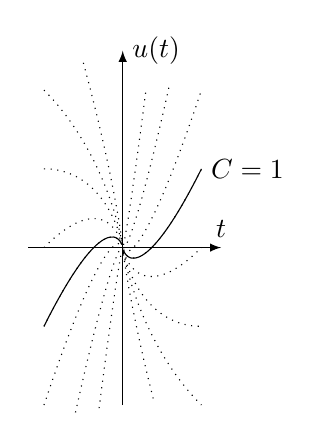
\begin{tikzpicture}
  \draw[-latex] (-1.2,0) -- (1.25,0) node [above] {\(t\)};
  \draw[-latex] (0,-2) -- (0,2.5) node [right] {\(u(t)\)};
  \draw[domain=-1:-0.01, variable=\t, samples=100] 
    plot( {\t}, {\t*(ln(-\t) + 1) } );
  \draw[domain=0.01:1, variable=\t, samples=100] 
    plot( {\t}, {\t*(ln(\t) + 1) } ) node[right] {\(C = 1\)};
                    %
  \foreach \c in {-2,-1,0,1,2}
  {
    \draw[domain=-1:-0.01, variable=\t, samples=100, dotted] 
      plot( {\t}, {\t*(ln(-\t) + \c) } );
    \draw[domain=0.01:1, variable=\t, samples=100, dotted] 
      plot( {\t}, {\t*(ln(\t) + \c) } );
  }
                    %
  \draw[domain=-0.6:-0.01, variable=\t, samples=100, dotted] 
    plot( {\t}, {\t*(ln(-\t) + 4) } );
  \draw[domain=0.01:0.6, variable=\t, samples=100, dotted] 
    plot( {\t}, {\t*(ln(\t) + 4) } );
                    %
  \draw[domain=-0.5:-0.01, variable=\t, samples=100, dotted] 
    plot( {\t}, {\t*(ln(-\t) - 4) } );
  \draw[domain=0.01:0.4, variable=\t, samples=100, dotted] 
    plot( {\t}, {\t*(ln(\t) - 4) } );
                    %
  \draw[domain=-0.3:-0.01, variable=\t, samples=100, dotted] 
    plot( {\t}, {\t*(ln(-\t) + 8) } );
  \draw[domain=0.01:0.3, variable=\t, samples=100, dotted] 
    plot( {\t}, {\t*(ln(\t)  + 8) } );
\end{tikzpicture}
\end{document}
